\documentclass{ikpKoeln}
\usepackage{graphicx}
\usepackage{physics}
\usepackage{xcolor}
\usepackage{tikz}
\usetikzlibrary{math}

\scTitle{Application of the Millepede algorithm to the Time and Position Calibration of NeuLAND}
\scAuthor{*}{Yanzhao}{Wang}{1}
\scAuthor{}{Igor}{Gasparic}{2}
\scAuthor{}{Håkan}{Johansson}{3}
\scAuthor{}{Andreas}{Zilges}{1}
\scAffiliation{1}{University of Cologne, Institute for Nuclear Physics, Germany}
\scAffiliation{2}{GSI Helmholtzzentrum für Schwerionenforschung, Germany}
\scAffiliation{3}{Chalmers University of Technology, Sweden}
\scEmail{ywang@ikp.uni-koeln.de}

\scTitleShort{Millepede algorithm for the Time and Position Calibration of NeuLAND}

\date{\scriptsize \today \\Conference\\Place Year}

\graphicspath{{../figures/}}

\addbibresource{reference.bib}

\begin{document}

\begin{frame}[t]{Title of this frame}
    \vspace*{-1em}
	\begin{columns}[t]
		\begin{column}{0.45\textwidth}
			\begin{block}{\small Some steps}
				\begin{itemize}
					\item<+-> Step 1
					\item<+-> Step 2
					\item<.-> Step 3
				\end{itemize}
			\end{block}
			\onslide<+->
			\begin{figure}
				\includegraphics[width=0.8\textwidth]{example-image-16x10}
			\end{figure}
		\end{column}
		\begin{column}{0.45\textwidth}
			\onslide<+->
			\begin{exampleblock}{Definition}
				Here goes the definition.
			\end{exampleblock}

			\begin{figure}
				\centering
				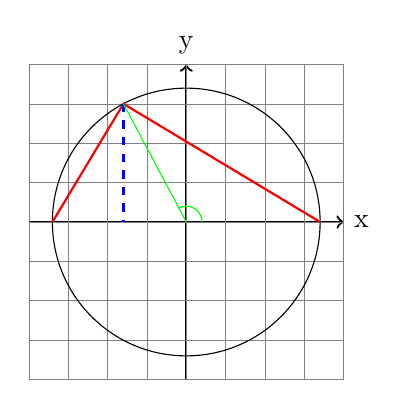
\begin{tikzpicture}
					\draw[->, thick, color = black] (-2, 0) -- (2, 0)node[right]{x};
					\draw[->, thick, color = black] (0, -2) -- (0, 2)node[above]{y};
					\draw[step = 0.5cm, very thin, color = gray] (-2, -2) grid (2, 2);
					\draw (0, 0) circle [radius = 1.7];

					\coordinate (aDot) at (118 : 1.7);
					\draw[color=red, thick] (-1.7, 0) -- (aDot) -- (1.7, 0);
                    \draw[color=blue, dashed, thick] (aDot) -- (aDot |- 0,0);
                    \draw[color=green] (aDot) -- ( 0,0);
                    \draw[color= green] (0.2 ,0) arc [start angle=0, end angle = 118, radius = 0.2];
				\end{tikzpicture}
				\caption{A random tikz graph}
			\end{figure}
		\end{column}
	\end{columns}
\end{frame}

\end{document}
